%=======================02-713 LaTeX template, following the 15-210 template==================
%
%
%
%
%    1. Update the information in section "A," put your name and the name of 
%       the class and the number of the problem set
%    2. Write your answers in section "B" below. Precede answers for all 
%       parts of a question with the command "\question{n}{desc}" where n is
%       the question number and "desc" is a short, one-line description of 
%       the problem. There is no need to restate the problem.
%    3. If a question has multiple parts, precede the answer to part x with the
%       command "\part{x}".
%

\documentclass[11pt]{article}
\usepackage[mathscr]{euscript}


\newcommand\question[2]{\vspace{.25in}\hrule\textbf{#1: #2}\vspace{.5em}\hrule\vspace{.10in}}
\renewcommand\part[1]{\vspace{.10in}\textbf{(#1)}}


% plots
\usepackage{graphicx}
\graphicspath{ {./images/} }


\usepackage{amsmath, amssymb, amsthm} %AMS packages
\usepackage{mathtools, graphicx, enumitem} %generally recommended
\usepackage{mathrsfs} %symbols I like
\usepackage{hyperref} %personal preference
\usepackage{microtype, } %recommended by stackexchange, never tried them myself
\usepackage{nag, todonotes} %workflow stuff, doesn't affect final document

% Layout
\usepackage{fancyhdr}
\usepackage[margin=1in]{geometry}
\lhead{\NAME}
\chead{\ClassNumber , Assignment \ANUM}
\rhead{Due: \duedate}
\setlength{\parindent}{0pt}
\setlength{\parskip}{5pt plus 1pt}
\setlength{\headheight}{13.6pt}
\pagestyle{fancyplain}


%-------------------------------------------<commands>--------------------------------------------------------
%%%%%%%%%%%%%%%%%%%%%%%%%%%%%%%%%%%%%%%%%											Letter Symbols
\newcommand{\R}{\mathbb{R}}
\newcommand{\N}{\mathbb{N}}
\newcommand{\Z}{\mathbb{Z}}
\newcommand{\Q}{\mathbb{Q}}
\newcommand{\C}{\mathbb{C}}
\newcommand{\F}{\mathcal{F}}
\renewcommand{\H}{\mathcal{H}} %overwrites long-umlaut diacritic
\newcommand{\eps}{\varepsilon}
\newcommand{\Exp}{\mathbb{E}}
\newcommand{\Info}{\mathcal{F}}
\renewcommand{\P}{\mathbb{P}}
%%%%%%%%%%%%%%%%%%%%%%%%%%%%%%%%%%%%%%%%%											Brackets
\newcommand{\paren}[1]{\left( #1 \right)}
\newcommand{\bracket}[1]{\left[ #1 \right]}
\newcommand{\chevron}[1]{\langle #1 \rangle}
\newcommand{\norm}[2][ ]{\left\lVert #2 \right\rVert_{#1}}
\newcommand{\abs}[1]{\left\lvert #1 \right\rvert}
\newcommand{\floor}[1]{\left\lfloor #1 \right\rfloor}
\newcommand{\ceil}[1]{\left\lceil #1 \right\rceil}
%%%%%%%%%%%%%%%%%%%%%%%%%%%%%%%%%%%%%%%%%											Operators
\DeclareMathOperator{\supp}{supp}
\DeclareMathOperator{\trace}{tr}
\DeclareMathOperator{\lspan}{span}
\DeclareMathOperator{\conv}{conv} % stands for conv, as in convex hull
\DeclareMathOperator{\Int}{int} % stands for int, as in interior of a set
\DeclareMathOperator{\cl}{cl}
\DeclareMathOperator{\sgn}{sgn}
\newcommand{\indep}{\perp \!\!\! \perp}
\newcommand{\NormCDF}[1]{\Phi \left[ #1 \right]}
%%%%%%%%%%%%%%%%%%%%%%%%%%%%%%%%%%%%%%%%%%											Aarows
\newcommand{\into}{\hookrightarrow}
\newcommand{\onto}{\twoheadrightarrow}
\newcommand{\weakly}{\rightharpoonup}
\newcommand{\isom}{\cong}
\newcommand{\restr}[1]{{\upharpoonright}_{#1}}
%\newcommand{\rest}{\big|}
%%%%%%%%%%%%%%%%%%%%%%%%%%%%%%%%%%%%%%%%%%											Common Abbreviations
\renewcommand{\th}{^\mathrm{th}} %overwrites thorn (old english letter)
\newcommand{\n}{^{-1}}
\newcommand{\half}{\frac{1}{2}}
%%%%%%%%%%%%%%%%%%%%%%%%%%%%%%%%%%%%%%%%%%											Differential Operators
\newcommand{\del}{\partial}
\newcommand{\grad}{\nabla}
\newcommand{\Laplace}{\Delta}
\renewcommand{\div}{\operatorname{div}} %overwrites division symbol
\newcommand{\dd}{\mathrm{d}}
\newcommand{\intd}{\,\dd}
\newcommand{\ddt}{\frac{\dd}{\dd t}}
\newcommand{\deriv}[2]{\frac{\dd #1}{\dd #2}} %can leave top blank, e.g. \deriv{}{x}
\newcommand{\pderiv}[2]{\frac{\partial #1}{\partial #2}} %ditto
%%%%%%%%%%%%%%%%%%%%%%%%%%%%%%%%%%%%%%%%%%											Favorite Functions and Space Names
\newcommand{\test}{\mathcal{D}}
\newcommand{\Ctest}{C_c^\infty}
\newcommand{\BMO}{\operatorname{BMO}}
\newcommand{\indic}[1]{\chi_{\{#1\}}}
\newcommand{\Leb}[2][\R^n]{L^{#2}(#1)}
%-------------------------------------------</commands>--------------------------------------------------------


\begin{document}\raggedright


%Section A==============Change the values below to match your information==================
\newcommand\NAME{Ki Hyun}  % your name
\newcommand\ClassNumber{FINM 36702}
\newcommand\ClassName{Portfolio Credit Risk: Modeling and Estimation}    
\newcommand\ANUM{3}              % the homework number
\newcommand\duedate{18:00 (CT) April 13th 2023}	% due date
%Section B==============Put your answers to the questions below here=======================

\title{Assignment \ANUM}
\author{\NAME \\ 
\ClassNumber \text{:} \ClassName}
\date{Due: \duedate}

\maketitle

%\question{1}{Description of problem}
%\part{a}

\question{1}{Default Rate and Loss Given Default}

The below two statements were given in the question

\begin{equation} \tag{1 - 1}
pdf_{dr}[dr] = 2 - 2dr
\end{equation}

\begin{equation}\tag{1 - 2}
lgd[dr] = dr^{\frac{1}{2}}
\end{equation}

From the two, we may infer the probability density function of $lgd$:

$$
\begin{aligned}
\P\{lgd \leq x\} &=
\P\{dr^{\frac{1}{2}} \leq x\} \\
&(\because \ (1 - 2), \ 0 \leq dr) \\
&= \P\{dr \leq x^2 \} \\
&= \begin{cases} 
\int_0^{x^2} (2 - 2dr) d(dr) & 0 \leq x \leq 1 \\
0 & \text{Otherwise}
\end{cases}
\\
&(\because (1 - 1), \ 0 \leq lgd \leq 1)
\end{aligned}
$$

Now focusing on the case where $0 \leq x \leq 1$:

$$
\begin{aligned}
\P\{lgd \leq x\} &=
\int_0^{x^2} (2 - 2dr) d(dr) \\
&= \left[ 
2dr - (dr)^2
\right]_0^{x^2} \\
&= (2x^2 - x^4) - 0 \\
&= 2x^2 - x^4
\end{aligned}
$$

$$
\begin{aligned}
\therefore
pdf_{lgd}[x] &= 
\frac{\delta}{\delta x} \P\{lgd \leq x\} \\
&= \frac{\delta}{\delta x} (2x^2 - x^4) \\
&= 4x - 4x^3 
\end{aligned}
$$

Ultimately, for $0 \leq lgd \leq 1$:

\begin{equation} \tag{1 - 3}
pdf_{lgd}[lgd] =
4 \cdot lgd - 4 \cdot (lgd)^3
\end{equation}

Now if we plot the two pdfs in (1 - 1) and (1 - 3) for the
range $(0, 1)$:

\begin{figure}[h]
\centering
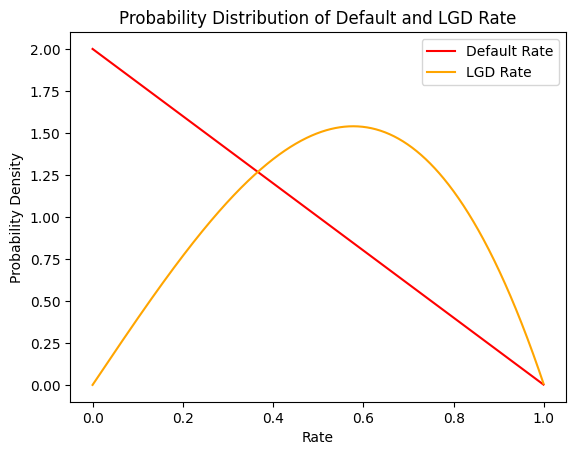
\includegraphics[scale=0.8]{Q1.png}
\caption{PDF of Default Rate and LGD}
\label{Fig:Q1}
\end{figure}

\newpage

\question{2}{Loss from Default Rate and Loss Given Default}

We know from definition that loss rate is the multiplication of
the default rate and the loss given default rate.

\begin{equation} \tag{2 - 1}
loss[dr, lgd] = dr \times lgd
\end{equation}

Now using the relationship given in (1 - 2), the loss function
becomes:

\begin{equation} \tag{2 - 1*}
loss[dr] = dr^{\frac{3}{2}}
\end{equation}

Similar to question 1, we can derive the probability density function
of loss rate using (2 - 1*) and (1 - 1):

$$
\begin{aligned}
\P\{loss \leq x\} &=
\P\{dr^{\frac{3}{2}} \leq x\} \\
&(\because (2 - 1*), \ 0 \leq dr) \\
&= \P\{dr \leq x^{\frac{2}{3}}\} \\
&= \begin{cases} 
\int_0^{x^{\frac{2}{3}}} (2 - 2dr) d(dr) & 0 \leq x \leq 1 \\
0 & \text{Otherwise}
\end{cases}
\\
&(\because (1 - 1), \ 0 \leq loss \leq 1)
\end{aligned}
$$

Now focusing on the case where $0 \leq x \leq 1$:

$$
\begin{aligned}
\P\{loss \leq x\} &=
\int_0^{x^{\frac{2}{3}}} (2 - 2dr) d(dr) \\
&= \left[ 
2dr - (dr)^2
\right]_0^{x^{\frac{2}{3}}} \\
&= (2x^{\frac{2}{3}} - x^{\frac{4}{3}}) - 0 \\
&= 2x^{\frac{2}{3}} - x^{\frac{4}{3}}
\end{aligned}
$$

$$
\begin{aligned}
\therefore
pdf_{loss}[x] &= 
\frac{\delta}{\delta x} \P\{loss \leq x\} \\
&= \frac{\delta}{\delta x} (2x^{\frac{2}{3}} - x^{\frac{4}{3}}) \\
&= \frac{4}{3} x^{-\frac{1}{3}} - \frac{4}{3} x^{\frac{1}{3}}
\end{aligned}
$$

Ultimately, for $0 \leq loss \leq 1$:

\begin{equation} \tag{2 - 2}
pdf_{loss}[loss] =
\frac{4}{3} \cdot (loss)^{-\frac{1}{3}} 
-\frac{4}{3} (loss)^{\frac{1}{3}}
\end{equation}

\newpage

Now if we plot the two pdfs in (1 - 1), (1 - 3), and (2 - 2) 
for the range $(0, 1)$:

\begin{figure}[h]
\centering
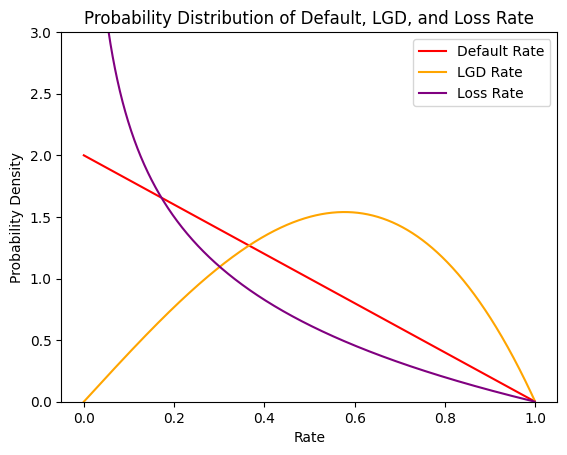
\includegraphics[scale=0.8]{Q2.png}
\caption{PDF of Default Rate, LGD, and Loss}
\label{Fig:Q2}
\end{figure}

\begin{itemize}
\item Expected Loss:

$$
\begin{aligned}
EL &= \Exp[loss] \\
&= \int_0^1 loss \cdot pdf_{loss}[loss] d(loss) \\
&= \int_0^1 loss 
\left( 
\frac{4}{3} \cdot (loss)^{-\frac{1}{3}} 
-\frac{4}{3} (loss)^{\frac{1}{3}}
\right) d(loss) \\
&= \int_0^1 \left( 
\frac{4}{3} \cdot (loss)^{\frac{2}{3}} 
-\frac{4}{3} (loss)^{\frac{4}{3}}
\right) d(loss) \\
&= \left[
\frac{4}{5} \cdot (loss)^{\frac{5}{3}} 
-\frac{4}{7} (loss)^{\frac{7}{3}}
\right]_0^1 \\
&= \left(\frac{4}{5} - \frac{4}{7} \right) - 0 \\
&= \frac{8}{35}
\end{aligned}
$$

\newpage

\item Expected Loss Given Default:

$$
\begin{aligned}
ELGD &= \frac{EL}{PD} \\
&= \frac{EL}{\int_0^1 dr \cdot pdf_{dr}[dr] d(dr)} \\
&= \frac{EL}{\int_0^1 dr \cdot (2 - 2dr) d(dr)} \\
&= \frac{EL}{\int_0^1 
\left(
2 \cdot dr - 2 \cdot (dr)^2 
\right) d(dr)} \\
&= \frac{EL}{
\left[
(dr)^2 - \frac{2}{3} (dr)^3
\right]_0^1} \\
&= \frac{EL}{
\left( 1 - \frac{2}{3} \right) - 0} \\
&= \frac{EL}{\frac{1}{3}} \\
&= \frac{24}{35}
\end{aligned}
$$


\item "Time-weighted" LGD:

$$
\begin{aligned}
EcLGD &= \Exp[cLGD] \\ 
&= \int_0^1 lgd \cdot pdf_{lgd}[lgd] d(lgd) \\
&= \int_0^1 lgd
\left(
4 \cdot lgd - 4 \cdot (lgd)^3
\right) d(lgd) \\
&= \int_0^1
\left(
4 \cdot (lgd)^2 - 4 \cdot (lgd)^4
\right) d(lgd) \\
&= \left[
\frac{4}{3} (lgd)^3 - \frac{4}{5} (lgd)^5
\right]_0^1 \\
&= \left(\frac{4}{3} - \frac{4}{5} \right) - 0 \\
&= \frac{8}{15}
\end{aligned}
$$
\end{itemize}

\newpage

\question{3}{Standard Deviation of a Vasicek Distribution}

Let $X$ follow a Vasicek distribution. Then, the standard deviation
becomes:

$$
\begin{aligned}
\sigma_X &= \sqrt{Var(X)} \\
&= \sqrt{\Exp[\left(X - \Exp[X] \right)^2]} \\
&= \sqrt{
\int_X (x - p)^2 \cdot pdf_X(x) dx} \\
&(\because \Exp[X] = p) \\
&= \sqrt{
\int_0^1 \sqrt{\frac{1 - \rho}{\rho}} (x - p)^2 
e^{
-\frac{1}{2 \rho} \left(
\sqrt{1 - \rho} \Phi^{-1}(x) - \Phi^{-1}(p)
\right)^2
+ \frac{1}{2} \left(
\Phi^{-1}(x)
\right)^2
} dx}
\end{aligned}
$$

Using the integration form above, we may plot the standard deviation
of the Vasicek distribution across $0.05 < \rho < 0.95$ for a
given $p = 0.10$:

\begin{figure}[h]
\centering
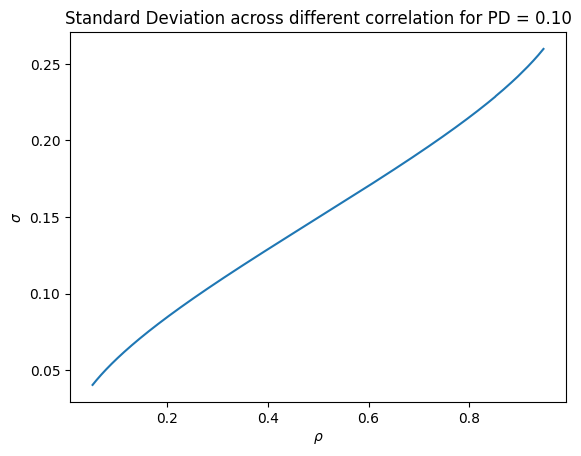
\includegraphics[scale=0.8]{Q3-1.png}
\caption{Std. Dev. of Vasicek vs $\rho$ for $PD = 0.10$}
\label{Fig:Q3-1}
\end{figure}

\newpage

The two Vasicek distributions ($Vasicek(p = 0.10, \rho = 0.05)$ and
$Vasicek(p = 0.10, \rho = 0.95)$) can be plotted as:

\begin{figure}[h]
\centering
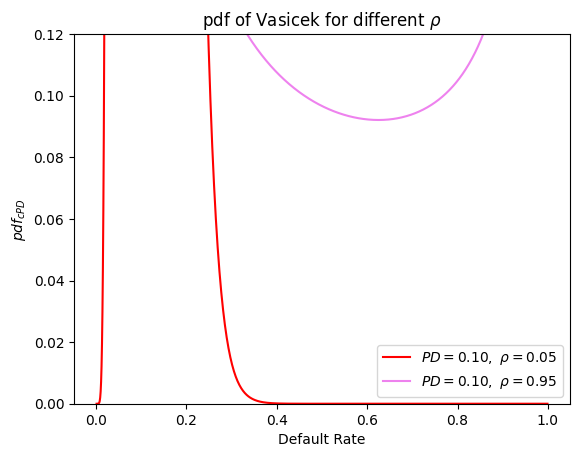
\includegraphics[scale=0.8]{Q3-2.png}
\caption{PDF of the two Vasicek Distribution}
\label{Fig:Q3-2}
\end{figure}

\newpage

\question{4}{Inverse CDF of Vasicek distribution}

Using the CDF of the Vasicek distribution:

\begin{equation} \tag{4 - 0}
F(x \mid p, \rho) = 
\Phi \left(
\frac{\sqrt{1 - \rho} \ \Phi^{-1}(x) - \Phi^{-1}(p)}
{\sqrt{\rho}}
\right)
\end{equation}

From the above CDF (4 - 0), the inverse CDF can be derived as:

\begin{equation} \tag{4 - 1}
F^{-1}(x \mid p, \rho) = 
\Phi \left(
\sqrt{\frac{\rho}{1 - \rho}} \Phi^{-1}(x)
+ \frac{1}{\sqrt{1 - \rho}} \Phi^{-1}(p)
\right)
\end{equation}

The two inverse CDFs may be plotted as below:

\begin{figure}[h]
\centering
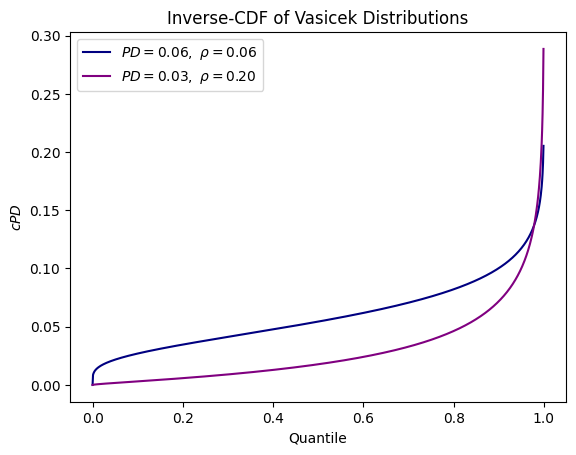
\includegraphics[scale=0.8]{Q4.png}
\caption{Inverse CDF Plot}
\label{Fig:Q4}
\end{figure}

Using optimization, the quantile at which both loans have
the same value of cPD can be estimated as $\approx 0.98$

\end{document}

$$
\begin{aligned}
\end{aligned}
$$